\documentclass[12pt, a4paper]{report}
%\documentclass[11pt, a4paper]{article}

%====================== PACKAGES ======================
\usepackage[french]{babel}

\frenchbsetup{StandardLists=true}
\usepackage{enumitem}
\usepackage{pifont}

\usepackage[utf8x]{inputenc}
%\usepackage[latin1]{inputenc}

%pour gérer les positionnement d'images
\usepackage{float}
\usepackage{amsmath}
\DeclareMathOperator{\dt}{dt}
\usepackage{amsfonts}
\usepackage{graphicx}
%\usepackage{tabularx}
\usepackage[colorinlistoftodos]{todonotes}
\usepackage{url}

%pour les informations sur un document compilé en PDF et les liens externes / internes
\usepackage[pdfborder=0]{hyperref}
\hypersetup{
	colorlinks = true
	}

%pour la mise en page des tableaux
\usepackage{array}
\usepackage{tabularx}
\usepackage{multirow}
\usepackage{multicol}
\setlength{\columnsep}{50pt}

%pour utiliser \floatbarrier
%\usepackage{placeins}
%\usepackage{floatrow}

%espacement entre les lignes
\usepackage{setspace}

%modifier la mise en page de l'abstract
\usepackage{abstract}

%police et mise en page (marges) du document
\usepackage[T1]{fontenc}
\usepackage[top=2cm, bottom=2cm, left=2cm, right=2cm]{geometry}

%Pour les galerie d'images
\usepackage{subfig}

\usepackage{pdfpages}

\usepackage{tikz}
\usetikzlibrary{trees}
\usetikzlibrary{decorations.pathmorphing}
\usetikzlibrary{decorations.markings}
\usetikzlibrary{decorations.pathreplacing,calligraphy}
%\usetikzlibrary{decorations}
\usetikzlibrary{angles, quotes}
\usepackage{verbatim}

\usepackage{appendix}

\usepackage{comment}

\usepackage{xcolor}

%\PreviewEnvironment{tikzpicture}
%\setlength\PreviewBorder{0pt}%

%====================== INFORMATION ET REGLES ======================

%rajouter les numérotation pour les \paragraphe et \subparagraphe
\setcounter{secnumdepth}{4}
\setcounter{tocdepth}{4}

\hypersetup{							% Information sur le document
pdfauthor = {Stephan Runigo},			% Auteurs
pdftitle = {Documentation},			% Titre du document
pdfsubject = {Documentation},		% Sujet
pdfkeywords = {Document},	% Mots-clefs
pdfstartview={FitH}}	% ajuste la page à la largeur de l'écran
%pdfcreator = {MikTeX},% Logiciel qui a crée le document
%pdfproducer = {} % Société avec produit le logiciel
%======================== DEFINITION COMMANDES ========================
\newcommand{\si}[1]{\textsf{\textit {#1}}}
\newcommand{\fsb}[1]{\textsf{\textbf {\footnotesize #1}}}
\newcommand{\ib}[1]{\item {\bf #1}}
\newcommand{\bi}[1]{\textbf{\textit {#1}}}
%======================== DEBUT DU DOCUMENT ========================
%
\begin{document}
%
%régler l'espacement entre les lignes
\newcommand{\HRule}{\rule{\linewidth}{0.5mm}}
%
% Titre, résumé, ... %
%
\begin{titlepage}
%
~\\[1cm]

\begin{center}
%\includegraphics[scale=0.5]{./presentation/chambreABulle}
\end{center}

\textsc{\Large }\\[0.5cm]

% Title \\[0.4cm]
\HRule

\begin{center}
{\huge \bfseries  La causalité\\
%titre 2\\[0.4cm]
 }
\end{center}

\HRule \\[1.5cm]

\begin{center}
%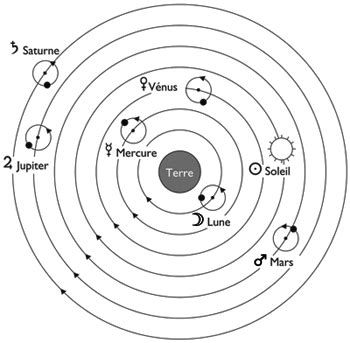
\includegraphics[scale=0.3]{./presentation/ptoleme}
\end{center}

\begin{center}
%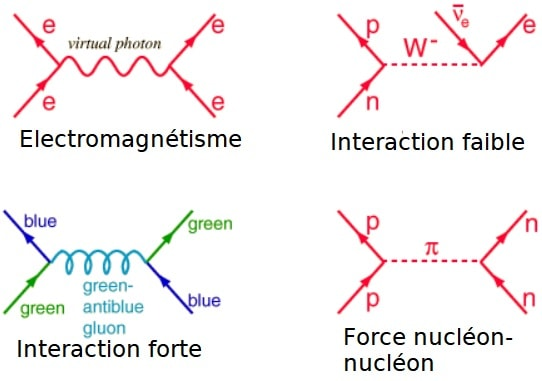
\includegraphics[scale=0.3]{./presentation/diagrammesInteractions}
\end{center}


% Author and supervisor
\begin{minipage}{0.4\textwidth}
\begin{flushleft} \large
%\emph{Auteur:}\\
%Stephan \textsc{Runigo}
\end{flushleft}
\end{minipage}
\begin{minipage}{0.4\textwidth}
\begin{flushright} \large
\emph{Auteur:}\\
Stephan \textsc{Runigo}
\end{flushright}
\end{minipage}

\vfill

% Bottom of the page
{\large \today}

\end{titlepage}

\newpage
\begin{center}
\Large
Résumé
\normalsize
\end{center}
\vspace{3cm}
\begin{itemize}[leftmargin=1cm, label=\ding{32}, itemsep=21pt]
\item {\bf Objet : } Souvenir des questions posés.
\item {\bf Contenu : } Définition, analyse, reflexion.
\item {\bf Public concerné : } Interressé à la question de l'âme.
\end{itemize}

\vspace{3cm}



\vspace{3cm}


%

%
% Table des matières
\tableofcontents
\thispagestyle{empty}
\setcounter{page}{0}
%
%espacement entre les lignes des tableaux
\renewcommand{\arraystretch}{1.5}
%
%====================== INCLUSION DES CHAPITRES ======================
%
~
\thispagestyle{empty}
%recommencer la numérotation des pages à "1"
\setcounter{page}{0}
\newpage
%\large
%
%%\section{B}
\chapter{}
%%{\bf }{\it }{\bf --} « » {\footnotesize X}$^\text{e}$
\section{Bigbang}

Lors des premiers instants du bigbang l'expansion de l'univers se serait produite à des vitesses supérieur à celle de la lumière.
Quelques instants plus tard, une transition de phase se serait produite transformant l'univers primordiale en un univers constitué de photon et d'autre particules.
Certaine de ces particule ayant une masse.
Cette transition de phase (ou une autre ?) aurait produit la masse en plus de fixer une vitesse limite.





{\footnotesize
\begin{itemize}[leftmargin=1cm, label=\ding{32}, itemsep=1pt]
\item {\bf \textsc{Étymologie} :} latin {\it },.
\item {\bf \textsc{Sens ordinaire} :} .
\item {\bf \textsc{Spiritualisme} :} .
\end{itemize}

\begin{itemize}[leftmargin=1cm, label=\ding{32}, itemsep=1pt]
\item {\bf \textsc{Terme voisin} :} .
\item {\bf \textsc{Terme opposé} :} .
\item {\bf \textsc{Corrélats} :} .
\end{itemize}
}

%%%%%%%%%%%%%%%%%%%
\section{}
%%%%%%%%%%%%%%%%%%%
{\footnotesize
\begin{itemize}[leftmargin=1cm, label=\ding{32}, itemsep=1pt]
\item {\bf \textsc{Étymologie} :} latin {\it },.
\item {\bf \textsc{Sens ordinaire} :} .
\item {\bf \textsc{Terme voisin} :} .
\item {\bf \textsc{Terme opposé} :} .
\item {\bf \textsc{Corrélats} :} .
\end{itemize}
}

\chapter{A}
%%{\bf }{\it }{\bf --}{\footnotesize X}$^\text{e}$
\section{Analogie}





\subsection{Incertitude}

Sécuriser son territoire, réduire l'incertitude, prendre une assurance,
car il y aurait un principe d'incertitude macroscopique.
Par analogie, on utilise abusivement ce terme en physique quantique

\subsection{Vibration}

Chronologiquement, l'Homme découvre le phénomène de la vibration.
Puis le caractère vibratoire au niveau quantique. Ce n'est pas parceque
la matière est fondamentalement vibratoire mais c'est parceque notre
entendement ne nous permet pas de comprendre la quantique. Notre
entendement nous mermet de distinguer le granulaire de l'ondulatoire.
Ni le granulaire ni l'ondulatoire ne sont vrai, la réalité est autre.
Si la théorie quantique parle d'onde et de corpuscule, c'est parceque
nous n'avons pas les capacités d'aller plus loin






{\footnotesize
\begin{itemize}[leftmargin=1cm, label=\ding{32}, itemsep=1pt]
\item {\bf \textsc{Étymologie} :} latin {\it },.
\item {\bf \textsc{Sens ordinaire} :} .
\item {\bf \textsc{Spiritualisme} :} .
\end{itemize}

\begin{itemize}[leftmargin=1cm, label=\ding{32}, itemsep=1pt]
\item {\bf \textsc{Terme voisin} :} .
\item {\bf \textsc{Terme opposé} :} .
\item {\bf \textsc{Corrélats} :} .
\end{itemize}
}

%\chapter{}
%%{\bf }{\it }{\bf --} « » {\footnotesize X}$^\text{e}$
\section{Bigbang}

Lors des premiers instants du bigbang l'expansion de l'univers se serait produite à des vitesses supérieur à celle de la lumière.
Quelques instants plus tard, une transition de phase se serait produite transformant l'univers primordiale en un univers constitué de photon et d'autre particules.
Certaine de ces particule ayant une masse.
Cette transition de phase (ou une autre ?) aurait produit la masse en plus de fixer une vitesse limite.





{\footnotesize
\begin{itemize}[leftmargin=1cm, label=\ding{32}, itemsep=1pt]
\item {\bf \textsc{Étymologie} :} latin {\it },.
\item {\bf \textsc{Sens ordinaire} :} .
\item {\bf \textsc{Spiritualisme} :} .
\end{itemize}

\begin{itemize}[leftmargin=1cm, label=\ding{32}, itemsep=1pt]
\item {\bf \textsc{Terme voisin} :} .
\item {\bf \textsc{Terme opposé} :} .
\item {\bf \textsc{Corrélats} :} .
\end{itemize}
}

%%%%%%%%%%%%%%%%%%%
\section{}
%%%%%%%%%%%%%%%%%%%
{\footnotesize
\begin{itemize}[leftmargin=1cm, label=\ding{32}, itemsep=1pt]
\item {\bf \textsc{Étymologie} :} latin {\it },.
\item {\bf \textsc{Sens ordinaire} :} .
\item {\bf \textsc{Terme voisin} :} .
\item {\bf \textsc{Terme opposé} :} .
\item {\bf \textsc{Corrélats} :} .
\end{itemize}
}

\chapter{C}
%
\section{Causalité}

Relation entre des phénomènes : deux phénomènes sont relié par
la causalité si l'un est la cause de l'autre.

Chez Hume, la croyance en une causalité est provoqué par l'habitude de voir deux phénomènes, l'un se produisant {\it systématiquement} avant l'autre. Le premier phénomène apparaissant est alors appelé {\it cause}, le second {\it effet}.

{\footnotesize
\begin{itemize}[leftmargin=1cm, label=\ding{32}, itemsep=1pt]
\item {\bf \textsc{Étymologie} :} latin {\it causa}, cause et
procés. latin {\it effectus}, résultat, effet, de {\it facere}, faire.
\item {\bf \textsc{Corrélats} :} déterminisme, temps.
\end{itemize}
}

%
\section{Causalité (principe de {\bf --})}

La cause précède l'effet.

Nous ne connaissons pas d'expérience remettant en cause ce
principe, la physique quantique décrit un univers causal.
{\footnotesize
\begin{itemize}[leftmargin=1cm, label=\ding{32}, itemsep=1pt]
\item {\bf \textsc{Corrélats} :} déterminisme, temps.
\end{itemize}
}

%
\section{Corpuscule}

petit grain de matière.
{\footnotesize
\begin{itemize}[leftmargin=1cm, label=\ding{32}, itemsep=1pt]
\item {\bf \textsc{Étymologie} :} latin {\it corpusculum}, de {\it corpus}, corps législatif, politique.
% 1495, J. de Vignay.
\item {\bf \textsc{Terme voisin} :} atome.
\item {\bf \textsc{Terme opposé} :} onde.
\item {\bf \textsc{Corrélats} :} substance.
\end{itemize}
}


\chapter{}
%%{\bf }{\it }{\bf --} « » {\footnotesize X}$^\text{e}$
\section{Durée}

Grandeur physique mesuré par un chronomètre.


Pour le physicien, le {\it temps} est l' « axe mathématique »
de la grandeur {\it durée}.



{\footnotesize
\begin{itemize}[leftmargin=1cm, label=\ding{32}, itemsep=1pt]
\item {\bf \textsc{Étymologie} :} latin {\it },.
\item {\bf \textsc{Sens ordinaire} :} .
\item {\bf \textsc{Spiritualisme} :} .
\end{itemize}

\begin{itemize}[leftmargin=1cm, label=\ding{32}, itemsep=1pt]
\item {\bf \textsc{Terme voisin} :} .
\item {\bf \textsc{Terme opposé} :} .
\item {\bf \textsc{Corrélats} :} .
\end{itemize}
}

\chapter{E}
%%{\bf }{\it }{\bf --} « » {\footnotesize X}$^\text{e}$
\section{Électron}
Particule élémentaire
{\footnotesize
\begin{itemize}[leftmargin=1cm, label=\ding{32}, itemsep=1pt]
\item {\bf \textsc{Étymologie} :} latin {\it electricus}, de {\it electrum}, du grec {\it êlektron}, ambre jaune, d'après sa propriété d'attirer les corps légers quand on l'a frotté.
% {\bf électron} 1829, Boiste, Stoney.
\item {\bf \textsc{Corrélats} :} proton, quanton.
\end{itemize}
}
\section{Énergie}
Grandeur physique.
{\footnotesize
\begin{itemize}[leftmargin=1cm, label=\ding{32}, itemsep=1pt]
\item {\bf \textsc{Étymologie} :} latin {\it energia}, du grec {\it energeia}, force en action.
% {\bf énergétique} du grec  {\bf energetikos}
%\item {\bf \textsc{Sens ordinaire} :} .
%\item {\bf \textsc{Spiritualisme} :} .
\item {\bf \textsc{Corrélats} :} temps.
\end{itemize}
}

%\input{./dico/F.tex}
\chapter{G}
%%{\bf }{\it }{\bf --}{\footnotesize X}$^\text{e}$
\section{Grandeur physique}

Résultat d'une {\it mesure expérimentale}.

Variable mathématique apparraissant dans les équations de la physique.

{\footnotesize
\begin{itemize}[leftmargin=1cm, label=\ding{32}, itemsep=1pt]
\item {\bf \textsc{Étymologie} :} latin {\it },.
\item {\bf \textsc{Sens ordinaire} :} .
\item {\bf \textsc{Spiritualisme} :} .
\end{itemize}

\begin{itemize}[leftmargin=1cm, label=\ding{32}, itemsep=1pt]
\item {\bf \textsc{Terme voisin} :} .
\item {\bf \textsc{Terme opposé} :} .
\item {\bf \textsc{Corrélats} : observable} .
\end{itemize}
}

%\input{./dico/H.tex}
\chapter{I}
%%{\bf }{\it }{\bf --}{\footnotesize X}$^\text{e}$
\section{Irréversible}

La physique statistique (ou thermodynamique) décrit les transformation des systèmes isolé comme irréversible : leur entropie augmente.

    Équation de Boltzmann
    


{\footnotesize
\begin{itemize}[leftmargin=1cm, label=\ding{32}, itemsep=1pt]
\item {\bf \textsc{Étymologie} :} latin {\it },.
\item {\bf \textsc{Sens ordinaire} : propriété du temps}.
\end{itemize}

\begin{itemize}[leftmargin=1cm, label=\ding{32}, itemsep=1pt]
\item {\bf \textsc{Terme voisin} :} .
\item {\bf \textsc{Terme opposé} :} .
\item {\bf \textsc{Corrélats} : temps} .
\end{itemize}
}

%\input{./dico/J.tex}
%\input{./dico/K.tex}
%\input{./dico/L.tex}
%\chapter{M}
%%{\bf }{\it }{\bf --} « » {\footnotesize X}$^\text{e}$
\section{Modèle}
Le fonctionnement d'un ordinateur peut servir de modèle afin de décrire le fonctionnement d'un humain. Il ne s'agit que d'un modèle, il ne prétend pas s'identifier à l'objet décrit. Il prétend donner une description relativement fidèle. Un bon paradigmme précise les limites de son modèle.
{\footnotesize
\begin{itemize}[leftmargin=1cm, label=\ding{32}, itemsep=1pt]
\item {\bf \textsc{} :} latin {\it modulus}, mesure.
\end{itemize}
}

\chapter{N}
%%{\bf }{\it }{\bf --} « » {\footnotesize X}$^\text{e}$
%%%%%%%%%%%%%%%%
\section{Neutre}
%%%%%%%%%%%%%%%%
Se dit d'un corps ne portant pas de charge électrique. Plus précisement, dont la charge électrique totale est nulle.
{\footnotesize
\begin{itemize}[leftmargin=1cm, label=\ding{32}, itemsep=1pt]
\item {\bf \textsc{Étymologie} :} latin {\it neuter}, ni l'un ni l'autre.
%{\bf neutron} 1932, Joliot.
%\item {\bf \textsc{Terme voisin} :} .
\item {\bf \textsc{Terme opposé} :} chargé électriquement.
\item {\bf \textsc{Corrélats} :} charge électrique.
\end{itemize}
}
%%%%%%%%%%%%%%%%%%
\section{Neutrino}
%%%%%%%%%%%%%%%%%%
Particule élémentaire.
Le neutrino est électriquement neutre.

En 2019, sa masse aurait été inférieur à 1,1 eV.
En 2022, sa masse serait inférieur à 0,8 eV.
En 2025, il serait possible qu'on en sache davantage sur sa masse
{\footnotesize
(https://www.quebecscience.qc.ca/sciences/mysterieuse-masse-neutrinos-katrin/)
}

{\footnotesize
\begin{itemize}[leftmargin=1cm, label=\ding{32}, itemsep=1pt]
\item {\bf \textsc{Étymologie} :} petit neutre (de l'italien ?) vers 1940.
\end{itemize}
}
%%%%%%%%%%%%%%%%%%
\section{Neutron}
%%%%%%%%%%%%%%%%%%
Particule pas si élémentaire (constitué de trois quarks).
Le neutron est électriquement neutre.
Sa masse est proche de celle du proton.
C'est un des constituants du noyau des atomes.
{\footnotesize
\begin{itemize}[leftmargin=1cm, label=\ding{32}, itemsep=1pt]
\item {\bf \textsc{Étymologie} :} neutre, {\bf neutron} 1932, Joliot.
\item {\bf \textsc{Corrélats} : proton, électron} .
\end{itemize}
}
%%%%%%%%%%%%%%%%
\section{Noumène}
%%%%%%%%%%%%%%%%
Objet de la raison, réalité intelligible {\bf --} Chose en soi.
{\footnotesize
\begin{itemize}[leftmargin=1cm, label=\ding{32}, itemsep=1pt]
\item {\bf \textsc{Étymologie} :} grec {\it nooumena}, choses pensées, {\it noumenon}, ce qui est pensée, {\it noein}, penser.
\item {\bf \textsc{Terme opposé} :} phénomène.
\end{itemize}
}

\chapter{}
%%{\bf }{\it }{\bf --} « » {\footnotesize X}$^\text{e}$
%%%%%%%%%%%%%%%%%%%%
\section{Observable}
%%%%%%%%%%%%%%%%%%%%
%\section{Physique quantique}
Opérateur mathématique associé à une grandeur physique.

L'observation d'un événement quantique correspond à une opération réalisé sur des quantons, changeant l'état de ces quantons.

{\footnotesize
\begin{itemize}[leftmargin=1cm, label=\ding{32}, itemsep=1pt]
\item {\bf \textsc{Étymologie} :} latin {\it observare} observer, veiller sur, respecter. {\it ob-} au-devant, {\it servare}, préserver, garder.
\item {\bf \textsc{Corrélats} :} Mesure.
\end{itemize}
}
%%%%%%%%%%%%%%
\section{Onde}
%%%%%%%%%%%%%%
Perturbation se propageant dans un milieux matériel.
{\footnotesize
\begin{itemize}[leftmargin=1cm, label=\ding{32}, itemsep=1pt]
\item {\bf \textsc{Étymologie} :} latin {\it unda}, vague, masse d'eau agité.
\item {\bf \textsc{Terme opposé :} corpuscule} .
\item {\bf \textsc{Corrélats :} dualité} .
\end{itemize}
}

\chapter{P}
%%{\bf }{\it }{\bf --} « » {\footnotesize X}$^\text{e}$
%%%%%%%%%%%%%%%%%%%%%%%%%%%%%%%
\section{Paradigme}
%%%%%%%%%%%%%%%%%%%%%%%%%%%%%%%
Ensemble (constituée de lois, de modèles et d'expériences) que l'on peut remettre en question.

La science est constituée de plusieurs paradigmes, certain concurrent entre eux, certains incompatibles entre eux.

{\footnotesize
\begin{itemize}[leftmargin=1cm, label=\ding{32}, itemsep=1pt]
\item {\bf \textsc{Étymologie} :} latin {\it parradigma}, (grec {\it paradeigma}), exemple,
de {\it deiknumi}, montrer.
% 1484, Chuquet.
\item {\bf \textsc{Terme voisin} :} théorie.
\item {\bf \textsc{Terme opposé} :} dogme.
\item {\bf \textsc{Corrélats} : science, révolution scientifique} .
\end{itemize}
}

%%%%%%%%%%%%%%%%%%%%%%%%%%%%%%%
\section{Particule élémentaire}
%%%%%%%%%%%%%%%%%%%%%%%%%%%%%%%
Se dit d'un quanton indivisible, ou du moins dont on ne connait pas de structure interne.
{\footnotesize
\begin{itemize}[leftmargin=1cm, label=\ding{32}, itemsep=1pt]
\item {\bf \textsc{Étymologie} :} latin {\it particula}, de {\it pars}, {\it partis}, partie.
% 1484, Chuquet.
{\bf élémentaire} 1390, Conty, du latin {\it elementarius}.
{\bf élément} latin {\it elementum}, principe, élément.
\item {\bf \textsc{Corrélats} : atome, quanton} .
\end{itemize}
}

%%%%%%%%%%%%%%%%
\section{Photon}
%%%%%%%%%%%%%%%%
Particule élémentaire, {\it quantum} de la lumière.
Le photon est électriquement neutre et sa masse est nulle.
{\footnotesize
\begin{itemize}[leftmargin=1cm, label=\ding{32}, itemsep=1pt]
\item {\bf \textsc{Étymologie} :} grec {\it phôs}, {\it phôtos}, lumière. 1923, Louis de Broglie.
\item {\bf \textsc{Corrélats} : lumière, électromagnétisme} .
\end{itemize}
}

%%%%%%%%%%%%%%%%
\section{Proton}
%%%%%%%%%%%%%%%%
Particule pas si élémentaire (constitué de trois quarks).
Le proton possède une charge électrique positive.
Sa masse est proche de celle du neutron.
C'est un des constituants du noyau des atomes.
{\footnotesize
\begin{itemize}[leftmargin=1cm, label=\ding{32}, itemsep=1pt]
\item {\bf \textsc{Étymologie} :} grec {\it prôton}, neutre de {\it prôtos}, premier. 1920, Rutherford.
\item {\bf \textsc{Corrélats} : neutron, électron, quanton} .
\end{itemize}
}

\chapter{}
%%{\bf }{\it }{\bf --} « » {\footnotesize X}$^\text{e}$
\section{Quanton}

entité décrite par son {\it vecteur d'état},

{\footnotesize
\begin{itemize}[leftmargin=1cm, label=\ding{32}, itemsep=1pt]
\item {\bf \textsc{Étymologie} :} latin {\it },.
\item {\bf \textsc{Sens ordinaire} :} .
\item {\bf \textsc{Spiritualisme} :} .
\end{itemize}

\begin{itemize}[leftmargin=1cm, label=\ding{32}, itemsep=1pt]
\item {\bf \textsc{Terme voisin} :} .
\item {\bf \textsc{Terme opposé} :} .
\item {\bf \textsc{Corrélats} :} .
\end{itemize}
}

\chapter{R}
%%{\bf }{\it }{\bf --}{\footnotesize X}$^\text{e}$
\section{Raisonnement}

\subsection{Raisonnement analytique}

Exemple : Tous les corps sont étendus : étendus est contenu dans l'idée de corps, a priori ()

\subsection{Raisonnement synthétique}

Exemple : Tous les corps sont pesants :  pesants n'est pas présent dans l'idée de corps, à postériori (C'est l'expérience qui nous l'apprend).

{\footnotesize
\begin{itemize}[leftmargin=1cm, label=\ding{32}, itemsep=1pt]
\item {\bf \textsc{Étymologie} :} latin {\it },.
\item {\bf \textsc{Sens ordinaire} :} .
\item {\bf \textsc{Spiritualisme} :} .
\end{itemize}

\begin{itemize}[leftmargin=1cm, label=\ding{32}, itemsep=1pt]
\item {\bf \textsc{Terme voisin} :} .
\item {\bf \textsc{Terme opposé} :} .
\item {\bf \textsc{Corrélats} :} .
\end{itemize}
}

%\chapter{S}
%%{\bf }{\it }{\bf --} « » {\footnotesize X}$^\text{e}$
\section{science}
Religion = idées que l'on ne peut pas remettre en question.

Science = idées que l'on peut remettre en question.

Exemple : la nature a horreur du vide (Aristote) -> pression atmosphérique (Torricelli 1643)
{\footnotesize
\begin{itemize}[leftmargin=1cm, label=\ding{32}, itemsep=1pt]
\item {\bf \textsc{Étymologie} :} latin {\it scientia}, de {\it electrum}, connaissance.
\end{itemize}
}

\chapter{T}
%%{\bf }{\it }{\bf --} « » {\footnotesize X}$^\text{e}$
\section{Temps}

La causalité quantique et l'irréversibilité thermodynamique
donnent deux {\it visions} du temps.

Pour le physicien, la durée est une grandeur physique, le
temps est l' « axe mathématique » de cette grandeur.

temps propre, durée de vie (de demi-vie)

{\footnotesize
\begin{itemize}[leftmargin=1cm, label=\ding{32}, itemsep=1pt]
\item {\bf \textsc{Étymologie} :} latin {\it },.
\item {\bf \textsc{Sens ordinaire} :} .
\item {\bf \textsc{Spiritualisme} :} .
\end{itemize}

\begin{itemize}[leftmargin=1cm, label=\ding{32}, itemsep=1pt]
\item {\bf \textsc{Terme voisin} : durée} .
\item {\bf \textsc{Terme opposé} :} .
\item {\bf \textsc{Corrélats} :} .
\end{itemize}
}

%%%%%%%%%%%%%%%%%%%
\section{Transition de phase}
%%%%%%%%%%%%%%%%%%%

Évolution brusque d'une grandeur thermodynamique ({\it température}, {\it pression}, {\it volume}).

Exemple de l'eau qui gèle : Lorsque l'on refroidie de l'eau liquide, il arrive un moment ou elle devient solide. Le passage de l'eau liquide à l'eau solide est une transition de phase : La température diminue de façon continue et si la pression reste constante, le volume augmente brusquement.

L'eau liquide est caractérisée par ses grandeurs physiques : {\it viscosité}, {\it tension superficielle}, {\it masse volumique}.

L'eau solide (la glace) est caractérisée par ses grandeurs physiques : {\it constante élastique}, {\it masse volumique}.

La glace possède une certaine viscosité mais à une echelle de temps très grande (on l'observe dans les glaciers). La viscosité de la glace est 10 millions de milliard de fois plus grande que celle de l'eau liquide. 

% eau : 10^-3 Pa s  glace : 10^13 Pa s  Vapeur d'eau 10,5 10^-5 Pa s

ANALOGIE

Lorsqu'en refroidissant, l'eau passe de l'état liquide à l'état solide, il apparaît une rigidité qui n'avait pas d'existence dans l'eau liquide. Apparait alors une constante de rigidité (tenseur des constantes élastiques)

Lors de l'expansion de l'univers, lors de la transition de phase, il apparaît une massité qui n'avait pas d'existence dans l'univers primordiale. Apparait alors une constante d'inertie (vitesse de la lumière, constante de la gravitation)

{\footnotesize
\begin{itemize}[leftmargin=1cm, label=\ding{32}, itemsep=1pt]
\item {\bf \textsc{Étymologie} :} latin {\it },.
\item {\bf \textsc{Sens ordinaire} :} .
\item {\bf \textsc{Terme voisin} :} .
\item {\bf \textsc{Terme opposé} :} .
\item {\bf \textsc{Corrélats} :} .
\end{itemize}
}

%\input{./dico/U.tex}
\chapter{V}
%%%%%%%%%%%%%%%%%%%
\section{Vibration}
%%%%%%%%%%%%%%%%%%%
Mouvement périodique.
{\footnotesize
\begin{itemize}[leftmargin=1cm, label=\ding{32}, itemsep=1pt]
\item {\bf \textsc{Étymologie} :} latin {\it vibrare}, agiter, brandir.
\item {\bf \textsc{Corrélats} : ondulatoire} .
\end{itemize}
}

%%%%%%%%%%%%%%%%%%%
\section{Vitesse}
%%%%%%%%%%%%%%%%%%%
{\footnotesize
\begin{itemize}[leftmargin=1cm, label=\ding{32}, itemsep=1pt]
\item {\bf \textsc{Étymologie} :} latin {\it },.
\item {\bf \textsc{Sens ordinaire} :} .
\item {\bf \textsc{Terme voisin} :} .
\item {\bf \textsc{Terme opposé} :} .
\item {\bf \textsc{Corrélats} :} .
\end{itemize}
}

%%%%%%%%%%%%%%%%%%%
\section{Vitesse de la lumière}
%%%%%%%%%%%%%%%%%%%

ANALOGIE
Lorsqu'en refroidissant, l'eau passe de l'état liquide à l'état solide, il apparaît une rigidité qui n'avait pas d'existence dans l'eau liquide.
Lors de l'expansion de l'univers, lors de la transition de phase, il apparaît une massité qui n'avait pas d'existence dans l'univers primordiale.



{\footnotesize
\begin{itemize}[leftmargin=1cm, label=\ding{32}, itemsep=1pt]
\item {\bf \textsc{Étymologie} :} latin {\it },.
\item {\bf \textsc{Sens ordinaire} :} .
\item {\bf \textsc{Terme voisin} :} .
\item {\bf \textsc{Terme opposé} :} .
\item {\bf \textsc{Corrélats} :} .
\end{itemize}
}

%\input{./dico/W.tex}
%\input{./dico/X.tex}
%\input{./dico/Y.tex}
%\input{./dico/Z.tex}

\chapter{Philosophie}

\section{Vocabulaire}
\newpage
\subsection{cause}
	\begin{itemize}[leftmargin=1cm, label=\ding{32}, itemsep=11pt]

\ib{Causalité} — \si{Épist.} Rapport de cause*
à effet. — Principe de causalité :
« Tout a une cause et, dans les
mêmes conditions, la même cause
est suivie du même effet. »

\ib{Cause} — \si{Méta.} {\bf 1.} Force$^2$ productrice,
engendrant l'effet et se prolongeant
en lui. {\it cf.} {\it Efficace}* et {\it Occasionnelle}*. — \si{Épist.} {\bf 2.} Antécédent$^1$
constant (Hume) et inconditionnel
(J. S. Mill). — {\bf 3.} Phénomène lié au
phénomène considéré par une relation fonctionnelle : « La cause n’est
jamais vraiment empirique » (Bachelard) $->$ {\it Dans la science}, l'explication par les forces productrices
(sens 1) fait place de plus en plus à
l’explication par les relations fonctionnelles (sens 3). Aussi, tandis
que F. Bacon disait que « savoir
vraiment, c’est savoir par les causes »
(sens 2), A. Comte a pu écrire
(Cours, I) que la science renonce à
la recherche des causes (sens 1), ce
qui est d'ailleurs auj. discuté.

—— \si{Hist.} {\bf 4.} {\it Aristote} distingue
4 espèces de causes : a) la cause matérielle ({\it p. e.} dans une statue, la
matière dont elle est faite); — b) la
cause formelle (la figure que la statue
représente; {\it cf.} Formel); — c) la
cause efficiente, {\it i. e.} la cause au sens 1
(le sculpteur); — d) la cause finale$^1$
(le but : désir de la gloire ou du gain,
visé par le sculpteur).

— \si{Méta.} {\bf 5.} Cause première : voir
Premier$^4$.

	\end{itemize}
\subsection{effet}
	\begin{itemize}[leftmargin=1cm, label=\ding{32}, itemsep=11pt]

\ib{Effet} — \si{Épist.} {\bf 1.} Phénomène considéré comme produit par
une cause efficiente*. — \si{Psycho.} {\bf 2.} Loi de
l'{\it effet} : celle qui pose que « toutes
% 62
choses égales d’ailleurs, une réponse
est renforcée par le succès, affaiblie,
éliminée, ou remplacée à la suite de l'échec » (Lagache).

\ib{Efficace} — \si{Méta.} Qui produit réellement son effet : « Cause efficace »
({\it opp.} « occasionnelle* »).

\ib{Efficience} — \si{Épist.} {\bf 1.} ({\it Opp.} : {\it finalité}*).
Causalité efficiente* : « La
science ne peut s'intéresser à la finalité qu'après avoir épuisé tout son
effort dans la découverte de l’efficience » (F. Houssay).

— \si{Vulg.} {\bf 2.} [Angl. : {\it efficiency}].
Rendement, effet utile : « Le pragmatisme* est une théorie de
l’efficience de la connaissance. »

\ib{Efficiente (Cause)} — Celle qui « produit » l'effet (cf.
{\it efficace}*). Cette expression s'emploie  {\it auj.} comme
syn. de {\it cause}* tout court (aux
sens 1, 2 et même 3), et par {\it opp.}
à {\it cause finale} (cf. {\it Cause}$^4$). {\it Chez
Aristote}, au ctr., la cause efficiente
se subordonne à la cause finale :
c’est « l’activité qui sort du fond
même de l’être et tend à réaliser la fin » (Goblot).

	\end{itemize}

\subsection{hasard}
	\begin{itemize}[leftmargin=1cm, label=\ding{32}, itemsep=11pt]

\ib{Hasard} — \si{Vulg.} Ce qui n’est pas prévisible : {\bf 1.} soit qu’on
suppose dans les choses une indétermination$^2$ radicale ; — {\bf 2.} soit
qu'il s'agisse d'événements si complexes (cf. {\it Fortuit}*) qu’on ne puisse
en connaître toutes les conditions : « Il n’y a pas incompatibilité entre le
rôle de ce que nous appelons le hasard et l’établissement de lois
scientifiques » (Borel) ; — {\bf 3.} soit qu’on ignore le déterminisme$^1$ du
phénomène ; — {\bf 4.} soit que, se plaçant au point de vue de la finalité*,
on n’en aperçoive
% 86
pas les raisons d’être : « Ce qui est hasard à l’égard des hommes
est dessein à l'égard de Dieu » (Bossuet). $->$ Terme très équivoque.

	\end{itemize}


\chapter{La causalité dans les sciences physiques}

%%%%%%%%%%%%%%%%%%%%%%%%%%%%%%%%%%%%%%%%%%%%

\section{Thermodynamique classique}

 \subsection{Doctrine du phlogistique}

Développée au {\footnotesize XVII}$^\text{e}$ siècle, 


Modèle : le phlogiston est décrit comme une substance {\it fluide}, contenue dans les matières combustibles et libérée	 lors de la combustion.

Le volume de cendre restant d'un volume de bois brulé justifie ce modèle. La masse supérieur, des oxydes métalliques obtenus par combustion des métaux était expliqué par l'attribution d'une masse négative au phlogiston.

 \subsection{Révolution énergétique}

Au {\footnotesize XVIII}$^\text{e}$ siècle, Antoine-Laurent Lavoisier conclut à l'inexistence du phlogiston grace à l'utilisation systématique de la balance dans l'étude des réactions chimiques.

Plusieurs modèles de la chaleur s'affrontent : la chaleur est une substance, avec ou sans masse. La chaleur est un type de mouvement, une vibration.

\texttt{ Émilio Segré, p 222 et suivantes}

Nouveau paradigme : la chaleur est une forme microscopique de l'énergie.

Nouveau principe : l'énergie se conserve, de l'énergie thermique peut se convertir en énergie mécanique, de l'énergie mécanique peut se convertir en énergie thermique, 

 \subsection{Entropie}
L'irréversibilité des transformations thermodynamique conduit à l'invention d'une nouvelle grandeur physique, l'entropie, ainsi qu'à l'énoncé du second principe de la thermodynamique : au cours d'une transformation d'un système isolé, l'entropie augmente.


 % \subsubsection{}

%%%%%%%%%%%%%%%%%%%%%%%%%%%%%%%%%%%%%%%%%%%




\chapter{La physique quantique}
%

%%%%%%%%%%%%%%%%%%%%%%%%%%%%%%%%%%%%%%%%%%%%

\section{Définitions}
  \subsection{Observateur et référentiel}

Pour étudier un mouvement, un {\it observateur} doit mesurer la position de l'objet en mouvement au cours du temps. Il doit donc disposer d'une horloge (pour mesurer le temps) et d'un système de coordonnées spatiales (pour mesurer la position).

L'horloge et le système de coordonnées "attachés" à l'observateur est appelé {\it référentiel}


    \subsubsection{Exemple}
Un observateur détermine la vitesse du train en chronomètrant la durée mis par le train pour parcourir la distance séparant les deux arbres.

\begin{center}
%\input{./relativiteMouvements/trainVapeur/train.tex}
\input{./relativiteMouvements/trainCorail/wagon.tex}
\end{center}

L'observateur est immobile par rapport à la Terre, le mouvement est étudié dans le {\it référentiel terrestre}.

Un voyageur est assis dans le train, il observe le paysage défiler. Il se trouve dans le {\it référentiel lié au train} et peut également chronométrer la durée pour parcourir la distance entre les deux arbres, et ainsi déterminer la "vitesse du paysage" dans son régérentiel.


  \subsection{Mouvement rectiligne uniforme}

Un mouvement {\it rectiligne} est un mouvement en ligne droite. Un mouvement {\it uniforme} est un mouvement dont la vitesse est constante.

%%%%%%%%%%%%%%%%%%%%%%%%%%%%%%%%%%%%%%%%%%%{\it }




%
%
%%%%%%%%%%%%%%%%%%%%%%%%%%%%%%%%%%%%%%%%%%%%

\section{Initiation au diagrammes de Feynman \cite{diagrammesFeynman}}

%%%%%%%%%%%%%%%%%%%%%%%%%%%%%%%%%%%%%%%%%%%

\label{JeanLucDeziel}

\subsection{Définition}

Un diagramme de Feynman est généralement un graphe en 2 dimensions où l'un des axe est attribué à l'espace, l'autre au temps, et dans lequel on représente les interactions entre les particules élémentaires. 
 %et dans lequel on représente les interactions entre les champs.

%Les champs échangent de l'énergie entre eux de manière quantique, à travers les phénomènes de création (ou émission) et d'anihilation (ou absorption) des quantons.

%On suppose que l'on dispose de dispositif expérimental permettant de détecter les particules.

Une vision corpusculaire (granulaire) des quantons permet de se familiariser avec ces diagrammes. Les diagrammes représentent alors les "trajectoires" des quantons.

L'électron et le photon sont des quantons. L'électron possède une masse ainsi qu'une charge électrique (il est l'un des principaux constituant de la matière avec le proton et le neutron). Le photon est la "particule de la lumière". Il n'a ni masse ni charge électrique et il se déplace à la vitesse de la lumière. Les interactions entre les électrons se produisent par échange de photon.


\subsection{Exemple et conventions}

Dans les diagrammes, un électron est représenté par un segment muni d'une flêche, un photon est représenté par un segment ondulé.

Dans les diagrammes suivants, les chiffres 1, 2, 3 et 4 ont été rajoutés pour des raisons pédagogiques, ils facilitent les explications chronologique des diagrammes.
\vspace{0.9cm}

\tikzset{
electron/.style={postaction={decorate}, decoration={markings,mark=at position .6 with {\arrow[#1]{latex}}}},
%positon/.style={postaction={decorate}, decoration={markings,mark=at position .5 with {\arrow[#1]{latex}}}},
photon/.style={decorate, decoration={snake, segment length=8pt, amplitude=1.8pt}}
}
\begin{minipage}[c]{.45\linewidth}
\begin{tikzpicture}
% désactive les caractères pour babel ? %\shorthandoff{:;!?};[scale=1.5]
\begin{scope}[scale=0.7]
%Création des axes xy
    \draw[-latex, very thick] (0,0) -- (5,0) node[below] {espace};
    \draw[-latex, very thick] (0,0) -- (0,5) node[left] {temps};
% Définition des noeuds
    \coordinate (e1) at (1,1);
    \coordinate (e2) at (4,2);
    \coordinate (e3) at (2,2.5);
   \coordinate (e4) at (1.3,4);
% dessin des particules
\draw [electron, very thick] (e1) -- (e3);
\draw [electron, very thick] (e3) -- (e4);
\draw [photon, very thick] (e3) -- (e2);
% Nommage
  \draw (e1) node [below] {1};
  \draw (e2) node [right] {2};
  \draw (e3) node [above right] {3};
  \draw (e4) node [above] {4};
\end{scope}
%above, below, right, left,
%above left, above right, below left, below right
%au-dessus, en-dessous, à droite, à gauche
%au-dessus à gauche, au-dessus à droite, en-dessous à gauche, en-dessous à droite
%
\end{tikzpicture}
\end{minipage}
\hfill
\begin{minipage}[c]{.45\linewidth}
\begin{center}
Explication chronologique :
\end{center}
Un électron se déplace de 1 à 3, un photon se déplace de 2 à 3. En 3, l'électron absorbe le photon. Muni de ce regain d'énergie, l'électron se précipite en 4.
\end{minipage}


\subsection{Interaction électromagnétique}

Les électrons sont des particules chargés électriquement'interaction entre deux électrons

%\vspace{1.1cm}
\begin{minipage}[c]{.45\linewidth}
\begin{center}
Explication chronologique :
\end{center}
Un électron se déplace de 1 à 3 tandis qu'un autre électron se déplace de 2 à 4.

\end{minipage}
\hfill
\begin{minipage}[c]{.45\linewidth}
\begin{tikzpicture}
% désactive les caractères pour babel ? %\shorthandoff{:;!?};
\begin{scope}[scale=0.7]
%Création des axes xy
   \draw[-latex, very thick] (0,0) -- (5,0) node[below] {espace};
   \draw[-latex, very thick] (0,0) -- (0,5) node[left] {temps};
% Définition des noeuds
   \coordinate (e1) at (2,1);
   \coordinate (e2) at (3.5,1);
   \coordinate (e3) at (1,4);
   \coordinate (e4) at (4,4);
% dessin des particules
\draw [electron, very thick] (e1) -- (e3);
\draw [electron, very thick] (e2) -- (e4);
% Nommage
  \draw (e1) node [left] {1};
  \draw (e2) node [right] {2};
  \draw (e3) node [left] {3};
  \draw (e4) node [right] {4};
\end{scope}
%above, below, right, left,
%above left, above right, below left, below right
%au-dessus, en-dessous, à droite, à gauche
%au-dessus à gauche, au-dessus à droite, en-dessous à gauche, en-dessous à droite
%
\end{tikzpicture}
\end{minipage}

%%%%%%%%%%%%%%%%%%%%%%%%%%%%%%%%%%%%%%%%%%%%%%%%%%%%%%%%%%%%%%%%%%%%%%%%%%%%%

%

%%%%%%%%%%%%%%%%%%%%%
\chapter{Paradigmes}
%%%%%%%%%%%%%%%%%%%%%

\section{Mécanique Newtoniennne}
%
La trajectoire d'un corps est décrite par ses coordonnées évoluant au cours du temps, obéissant au lois de la mécanique.
%
\section{Mécanique quantique}

L'évolution au cours du temps d'un quanton est décrite par sa fonction d'onde donnant l'amplitude de probabilité de mesurer ce quanton (de l'observer). La fonction d'onde evolue suivant l'équation de Schrödinger.

\section{Théorie quantique des champs}

Les différents champs échangent de l'énergie entre eux de manière quantique.

%%%%%%%%%%%%%%%%%%%%%%%%%%%%%%%%%%%%%%%%%%%%%%%%%%%%%%%%%%%%%%%%%%%%%%%%%%%%%%%%%%%%%

%
%
%%%%%%%%%%%%%%%%%%%%%%%%%%%%%%%%%%%%%%%%%%%%

\section{Théorie des champs}

%%%%%%%%%%%%%%%%%%%%%%%%%%%%%%%%%%%%%%%%%%%

%\subsection{}

Finallement, le diagramme représentant un échange élémentaire d'énergie entre le champ électron et le champ photon est le suivant :

\begin{center}
\includegraphics[scale=2.5]{./quantique/feynmannElementaire}
\end{center}

Un tel échange se représente comme un processus unique qui apparaît tantôt comme une création, tantôt comme une anihilation, tantôt comme une émission, tantôt comme une absorption, suivant comment on place les axes de temps et d'espace.

%Ainsi, il semblerait que ce processus élémentaire d'interaction entre les champs se produirait sans existence prélable de temps et d'espace, mais faisant apparaître un temps et un espace à nos sens.

\subsection{Champs et quantons}

Les quantons n'apparaissent alors plus comme des "particules de matière" mais comme la "signature" des champs échangeant de l'énergie.

L'électromagnétisme quantique décrit donc les champs photon, électron et positron, comme trois champs "couplés". Ce couplage signifie qu'ils échangent de l'énergie entre eux. Cet échange se produit de façon quantique (quantifié, discrète, "atomique").

La nature nous apparaitrait comme quantifié car nous considérons comme "objet", non pas les champs, mais leurs échanges, leur couplage. La nature serait constitué de champs, continus, leur interaction discontinu nous faisant apparaître une nature "atomique".  

\subsection{Espace-temps et causalité}

Le diagramme élémentaire nous montre une unification des interactions entre les champs, dans laquelle l'espace et le temps jouerait un rôle "secondaire". On aurait plutôt à faire à des "évènements espacé" (échange quantique entre les champs) qui vérifiraient un "principe causal". L'espace-temps serait alors notre perception de ce monde d'évènements "espacés et causaux". en effet :

Ce qui ressort de l'espace-temps des physiciens, c'est principalement l'invariance de la vitesse de la lumière, l'espace et le temps sont reliés, ce qui est fondamental semble être leur "liens", la vitesse limite.

La vitesse limite peut apparaître comme la "signature" d'un principe de causalité auquel obéirait les champs.
%%%%%%%%%%%%%%%%%%%%%%%%%%%%%%%%%%%%%%%%%%%%%%%%%%%%%%%%%%%%%%%%%%%%%%%%%%%%%

%
%\input{./quantique/feynmann.tex}
%
%


\section{Physique statistique}
%\newpage

Le principe "Les mêmes causes produisent les mêmes effets" est retrouvé grâce à la physique statistique : il ne s'agit plus d'un principe fondamental, que l'on choisit de poser, mais d'un théorème que l'on démontre. 


\section{Physique relativiste}

Le postulat de la physique relativiste est : "Les lois de la physique sont les mêmes dans tout les référentiels". On peut en déduire : "La vitesse de la lumière est une constante", "La vitesse de la lumière est une vitesse limite". Autrement dit, rien ne peut aller plus vite que la lumière. La vitesse de la lumière se note c, sa valeur est 300 000 km/s.

Cette vitesse limite, restreint le principe de causalité. En effet, considérons deux évènement A et B, distant l'un de l'autre, et supposons que A est la cause de B. L'évènement B ne peut donc avoir lieu qu'après avoir été prévenu que l'évenement A a eu lieu. Il faut donc "un messager" prévenant B que A a eu lieu, ce messager ne pouvant aller plus vite que la lumière, B ne peut avoir lieu qu'après un certain laps temps incompressible le séparant de A

Ainsi, dans le paradigme de la relativiré restreinte, le principe de causalité est modifié : "L'effet à lieu après un temps incompressible de la cause".



%Dans le paradigme de la relativiré restreinte, un objet, possédant une masse, ne peut pas dépasser la vitesse de la lumière. La lumière se propage à la vitesse de la lumière. Ainsi, un photon, un signal lumineux, vont nécessairement à la vitesse

%\subsection{Relativisme}
%(À distinguer du relativisme : "Les opinions sont subjectifs").





%
%\input{./chapitre2/chapitre2.tex}
%
%====================== INCLUSION DE LA BIBLIOGRAPHIE ======================
%
%récupérer les citation avec "/footnotemark" : 
\nocite{*}
%
% choix du style de la biblio
\bibliographystyle{plain}
%
% inclusion de la biblio
\cleardoublepage
\addcontentsline{toc}{chapter}{Bibliographie}
\bibliography{bibliographie.bib}
%
%====================== FIN DU DOCUMENT ======================
%
\end{document}
%%%%%%%%%%%%%%%%%%%%%%%%%%%%%%%%%%%%%%%%%%%%%%%%%%%%%%%%%%%%%%%%%%%%%%%%%%%%%%%%%
